% Povinný argument: Kód předmětu
\newcommand{\subject}{MPC-TVP}
% Povinný argument: Název předmětu
\newcommand{\subjectname}{SZZ}
% Povinný argument: Seznam autorů
\newcommand{\authors}{--}
% Povinný argument: Seznam korektorů
\newcommand{\corrections}{--}
% Nepovinný argument: Popis dokumentu
\newcommand{\docdesc}{Vypracované otázky k SZZ 2022}
% Nepovinný argument: Cílová skupina dokumentu
\newcommand{\docgroup}{Mikroelektronika, FEKT VUT}
% Nepovinný argument: URL repozitáře nebo jiný odkaz na dokument
\newcommand{\docurl}{}

% Přepsáním argumentu na 'false' vypnete balíček 'minted' pro sázení kódu.
% Pro jeho použití lokálně musíte mít v systému dostupný Python 3, python
% knihovnu 'minted' a PDFLaTeX musíte spouštět s argumentem '-shell-escape'.
% Místo něj můžete použít prostředí 'lstlisting'.
\newcommand{\docminted}{false}

% FEKT.tex
% https://github.com/VUT-FEKT-IBE/FEKT.tex
% Git hash repozitáře v době kopírování:

\documentclass[
    % Velikost základního písma je 12 bodů
    12pt,
    % Formát papíru je A4
    a4paper,
    % Oboustranný tisk
    twoside,
    % Záložky a metainformace ve výsledném PDF budou v kódování unicode
    unicode,
]{article}

%%%%%%%%%%%%%%%%%%%%
% OBECNÉ NASTAVENÍ %
%%%%%%%%%%%%%%%%%%%%

% Kódování zdrojových souborů
\usepackage[utf8]{inputenc}
% Kódování výstupního souboru
\usepackage[T1]{fontenc}
% Podpora češtiny
\usepackage[czech]{babel}

% Geometrie stránky
\usepackage[
    % Horní a dolní okraj
    tmargin=25mm,
    bmargin=25mm,
    % Vnitřní a vnější okraj
    lmargin=30mm,
    rmargin=20mm,
    % Velikost zápatí
    footskip=17mm,
    % Vypnutí záhlaví
    nohead,
]{geometry}

% Zajištění kopírovatelnosti a prohledávanosti vytvořených PDF
\usepackage{cmap}
% Podmínky (pro použití v titulní straně)
\usepackage{ifthen}

%%%%%%%%%%%%%%%
% FORMÁTOVÁNÍ %
%%%%%%%%%%%%%%%

% Nastavení stylu nadpisů
\usepackage{sectsty}
% Formátování obsahů
\usepackage{tocloft}
\setcounter{tocdepth}{1}
% Odstranění mezer mezi řádky v seznamech
\usepackage{enumitem}
\setlist{nosep}
\setitemize{leftmargin=1em}
\setenumerate{leftmargin=1.5em}
\renewcommand{\labelitemi}{--}
\renewcommand{\labelitemii}{--}
\renewcommand{\labelitemiii}{--}
\renewcommand{\labelitemiv}{--}
% Sázení správných uvozovek pomocí '\enquote{}'
\usepackage{csquotes}
% Vynucení umístění poznámek pod čarou vespod stránky
\usepackage[bottom]{footmisc}
% Automatické zarovnání textu k předcházení vdov a parchantů
\usepackage[defaultlines=3,all=true]{nowidow}
% Zalomení části textu pokud není na současné stránce dost místa
\usepackage{needspace}
% Nastavení řádkování
\usepackage{setspace}
\onehalfspacing
% Změna odsazení odstavců
\setlength{\parskip}{1em}
\setlength{\parindent}{0em}

% Bezpatkové sázení nadpisů
\allsectionsfont{\sffamily}
% Změna formátování nadpisu a podnadpisů v Obsahu
\renewcommand{\cfttoctitlefont}{\Large\bfseries\sffamily}
\renewcommand{\cftsubsecdotsep}{\cftdotsep}

% Použití moderní/aktualizované sady písem
\usepackage{lmodern}

%%%%%%%%%%%
% NADPISY %
%%%%%%%%%%%

\usepackage{titlesec}

\titlespacing*{\section}{0pt}{10pt}{-0.2\baselineskip}
\titlespacing*{\subsection}{0pt}{0.2\baselineskip}{-0.2\baselineskip}
\titlespacing*{\subsubsection}{0pt}{0.2\baselineskip}{-0.2\baselineskip}
\titlespacing*{\paragraph}{0pt}{0pt}{1em}

%%%%%%%%%%
% ODKAZY %
%%%%%%%%%%

% Tvorba hypertextových odkazů
\usepackage[
    breaklinks=true,
    hypertexnames=false,
]{hyperref}
% Nastavení barvení odkazů
\hypersetup{
    colorlinks,
    citecolor=black,
    filecolor=black,
    linkcolor=black,
    urlcolor=blue
}

%%%%%%%%%%%%%%%%%%%%%%%%%%%
% OBRÁZKY, GRAFY, TABULKY %
%%%%%%%%%%%%%%%%%%%%%%%%%%%

% Vkládání obrázků
\usepackage{graphicx}
\usepackage{subfig}
% Nastavení popisů obrázků, výpisů a tabulek
\usepackage{caption}
\captionsetup{justification=centering}
% Grafy a vektorové obrázky
\usepackage{tikz}
\usetikzlibrary{shapes,arrows}
% Složitější tabulky
\usepackage{tabularx}
\usepackage{multicol}

% Sázení osamocených float prostředí v horní části stránky
\makeatletter
\setlength{\@fptop}{0pt plus 10pt minus 0pt}
\makeatother

% Vynucení vypsání floating prostředí pomocí \FloatBarrier
\usepackage{placeins}

%%%%%%%%%%%%%%
% MATEMATIKA %
%%%%%%%%%%%%%%

% Sázení matematiky a matematických symbolů ('\mathbb{}')
\usepackage{amsmath}
\usepackage{amssymb}
% Sázení fyzikálních veličin
\usepackage{siunitx}

%%%%%%%%%%%%%%%%%
% ZDROJOVÉ KÓDY %
%%%%%%%%%%%%%%%%%

% Sazba zdrojových kódů
\usepackage[formats]{listings}
% Přepnutí prostředí 'code' do režimu výpisu kódu
\newenvironment{code}{\captionsetup{type=listing}}{}

% Balíček 'minted' budeme používat pouze pokud je jeho hodnota nastavena na 'true'
\providecommand{\docminted}{false}
\ifthenelse{\equal{\docminted}{true}}
{
    % Sazba zdrojových kódů
    \usepackage[newfloat]{minted}
    % Nastavení barev 'minted' kódů
    \usemintedstyle{pastie}
}
{
    % \docminted není 'true', nic neprovádíme
    % Pokud je v dokumentu 'minted' prostředí, dokument se nepodaří přeložit.
}
%%%%%%%%%%%
% TITULKA %
%%%%%%%%%%%

\IfFileExists{./.repo.tex}{
    % Soubor '.repo.tex' může (re)definovat povinné a nepovinné argumenty
    % souboru 'main.tex'. To lze využít v případech kdy v jednom repozitáři
    % existuje více dokumentů najednou (např. státnicové otázky).
    \input{.repo}
}{}

% Pokud byly nepovinné argumenty zakomentovány nebo vymazány, přidáme prázdné
% definice příkazů, aby bylo dokument možné správně přeložit.
\providecommand{\docdesc}{}
\providecommand{\docgroup}{}
\providecommand{\docurl}{}

\newcommand{\titulka}{
    \vspace*{2em}
    \begin{center}
        {\Huge \bfseries \subject}

        \vspace*{1em}

        {\Huge \bfseries \subjectname}

        \vspace*{2em}

        {\Large \docdesc}

        \vspace*{1em}

        \docgroup

        \url{\docurl}
    \end{center}

    \vfill

    \begin{tabular}{ll}
        Text:      & \authors     \\
        Korektura: & \corrections \\
    \end{tabular}
    \hfill
    \today

    \thispagestyle{empty}
    \newpage
}


\begin{document}

\titulka{}

\tableofcontents
\thispagestyle{empty}

\setcounter{page}{0}

\section{DVOJRAMPOVÝ OSCILÁTOR S VCO CHARAKTERISTIKOU}
Nastaveni střídy oscilátoru, výpočet kmitočtu oscilátoru, nastavení minimální a maximální frekvence oscilátoru s ohledem na řídící napětí

\begin{figure}[h]
   \begin{center}
     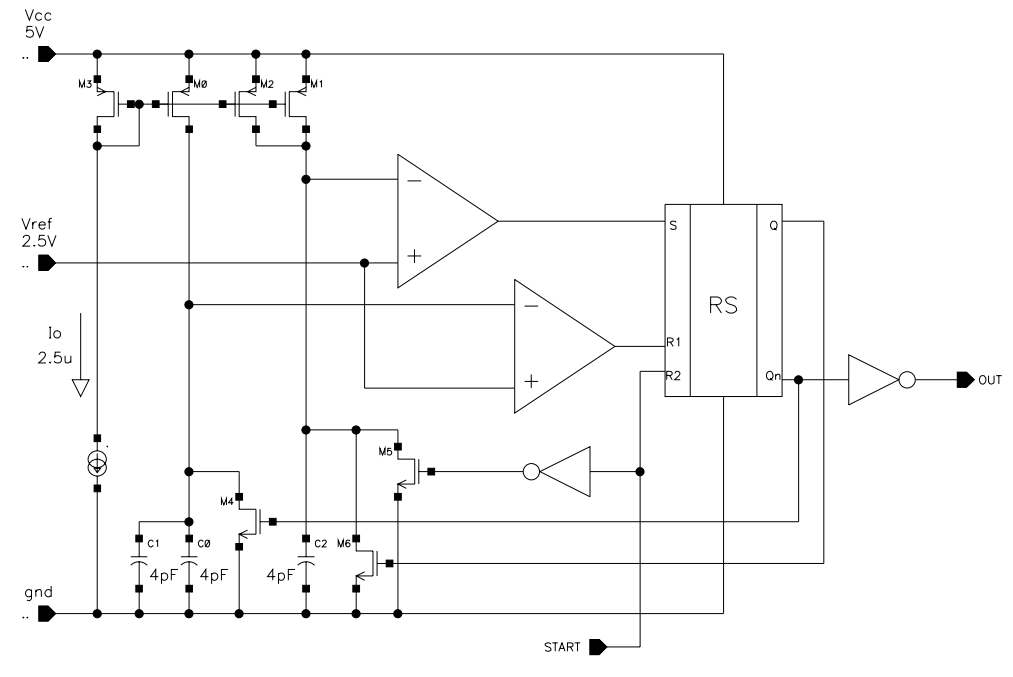
\includegraphics[scale=0.4]{images/OSC.png}
   \end{center}
   \caption{Dvourampový oscilátor}
\end{figure}

\subsection{Výpočet kmitočtu a nastavení střídy}

\begin{equation}
T_{1} = \frac{U_{ref}*C}{I}
\end{equation}
U této části periody se uplatňuje dvojice paralelních kondenzátorů, výsledná kapacita tedy bude 2*4 pF = 8 pF. Proud přes PMOS proudové zrcadlo se pouze zrcadlí jedenkrát,tedy I = 2,5 $\mu$A. 
\begin{equation*}
T_{1} = \frac{2,5*8*10^{-12}}{2,5*10^{-6}} = 8 us
\end{equation*}

Pro druhou část periody platí analogicky totéž, ovšem pro jiné hodnoty (viz. schéma).

\begin{equation*}
T_{2} = \frac{U_{ref}*C}{I} = \frac{2,5*4*10^{-12}}{5*10^{-6}} = 2 us
\end{equation*}

Kmitočet se poté vypočítá z převrácené hodnoty celé periody:

\begin{equation*}
f = \frac{1}{T_{1}+T_{2}} =  \frac{1}{8*10^{-6}+2*10^{-6}} = 100 kHz
\end{equation*}

\section{MANAGEMENT NAPÁJECÍHO NAPĚTÍ INTEGROVANÉHO OBVODU}
UVLO (řízení obvodu pomocí vstupního napájecího napětí, komparace vstupního napětí), Power on Reset (UV signál), realizace a výpočet nastaveni komparačních úrovní

\begin{figure}[h]
   \begin{center}
     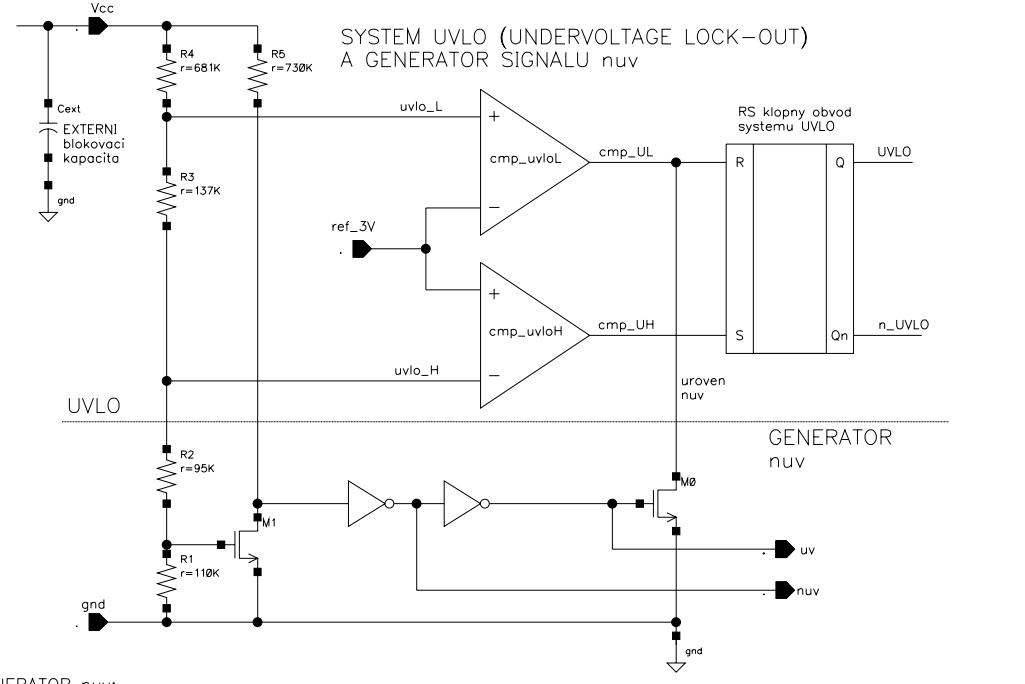
\includegraphics[scale=0.5]{images/UVLO.png}
   \end{center}
   \caption{Systém UVLO}
\end{figure}

\subsection{UVLO}
UVLO systém se aktivuje, pokud napájecí napětí Ucc dosáhne "zespodu" hodnoty UccH a zablokuje (disable) IO pokud napětí poklesne pod UccL. Po zapnutí se na Ucc pinu objeví lenárně rostoucí napětí. Na začátku je hodnota uvloL i uvloH nižší než 3 V, což způsobí, že výstup komparátoru cmpUVLOL je v úrovni L a výstup komparátoru cmpUVLOH je v úrovni H. Nízká úroveň compUVLOL na výstupu vyresetuje RS klopný obvod, na jeho Q výstupu se objeví nízká úroveň, která blokuje IO. Napětí Ucc pak dosáhne takové úrovně, že je vyšší, než komparační napětí 3 V, což způsobí přechod komparátoru compUVLOL do stavu H.

Napětí na vstupu uvloH je zatím nižší než 3 V, na výstupu komparátoru compUVLOH je stále úroveň H a funkce IO je blokovaná. Pokud hodnota Ucc dosáhne takové úrovně UccH, že napětí na vstupu uvloH přesáhne úroveň 3 V, přejde vstup komparátoru cmpUVLOH do úrovně L a změní se stav RS obvodu, na výstupu Q se objeví stav High, což odblokuje IO.

Pokud napětí Ucc klesne pod úroveň UccH, přejde Q klopného RS obvodu do H, ale RS obvod si stále pamatuje svůj předchozí stav a IO není blokován. 

Pokud napětí Ucc klesne pod UccL, přejde výstup komparátoru cmpUVLOL do stavu L, což změní stav klopného RS obvodu a na výstupu Q se objeví stav L a IO je tak blokován. 

Úrovně UccH a UccL se vypočítají následovně:

\begin{equation}
Ucc_{H} = U_{ref}*\frac{R_{1}+R_{2}+R_{3}+R_{4}}{R_{1}+R_{2}}
\end{equation}

\begin{equation}
Ucc_{L} = U_{ref}*\frac{R_{1}+R_{2}+R_{3}+R_{4}}{R_{1}+R_{2}+R_{3}}
\end{equation}

\subsection{Signál UV}
Signál UV slouží k nastavení vnitřní logiky celého systému při zapnutí napájecího napětí. Předpokládá se, že napájecí napětí je blokováno kondenzátorem, takže náběh napětí Ucc je poměrně pomalé. Při zapnutí narůstá na pinu Ucc napětí. Pokud je jeho hodnota nízká, tak NMOS M1 je zavřený a na jeho drainu je úrověň H a signál NUV je na úrovni L.

Nízkou úroní signálu NUV se nastaví (resetuje) logika celého IO. Signál NUV přejde do úrovně H a okamžiku, kdy napětí na pinu Ucc dosáhne takové úrovně, že tranzistor M1 sepne z H do L (signál NUV z L do H) je určena prahová hodnota napětí Ugs = Ugsr tranzistoru M1, při níž M1 sepne dělič R1 až R4.

Prahová hodnota Ugs je asi Ugsr = 0,85 V. Z tohoto se určí hodnota Uccr při níž signál NUV přechází z L do H.

\begin{equation}
U_{ccr} = U_{gsr}*\frac{R_{1}+R_{2}+R_{3}+R_{4}}{R_{1}}
\end{equation}

\section{Filtrační obvody}
-funkce, příklady realizací, důvody použití v převodnících, aproximační charakteristiky, přesné filtry.

\subsection{Funkce}
Jedná se obvykle o filtry typu dolní propust.
Je určen k:
\begin{itemize}
\item potlačování záznějí (Aliasing) – omezení šířky pásma vstupního signálu,
\item  potlačení kvantovacího šumu na výstupu DAC
\item a potlačení střídavých složek v nepřímých převodnících DA.
\end{itemize}

Problém aliasingu (záznějí) je vidět na obrázku \ref{fig:ali}, kde vstupní analogový signál má kmitočtovou odezvu (\ref{fig:ali}a)) a kmitočet f\textsubscript{b} je maximální kmitočet vstupního signálu. Pokud je vstupní analogový signál vzorkován s vzorkovacím kmitočtem f\textsubscript{s} je kmitočnotá odezva tohoto signálu jako na \ref{fig:ali}b).

Spektrum vstupníhosignálu se zrcadlí na kmitočtu f\textsubscript{s} a každé jeho vyšší harmonické složce. Pokud ale f\textsubscript{b} přesáhne polovinu f\textsubscript{b}, dojde k částečnému překrytí postranních složek, viz \ref{fig:ali}c). V důsledku toho pak může dojít k významné ztrátě informace o původním signálu, který pak již nelze rekonstruovat do původní podoby.

Proto musí být dodržen vzorkovací teorém:
\begin{equation}
 f_{s} > 2*f_{b}
\end{equation}

Uvedený vztah platí pouze pro harmonický signál resp. nejvyšší harmonickou složku jiného signálu. Antialiasingový filtr je použit proto, aby zabránil překrytí postranních složek, \ref{fig:ali}d)

   \begin{figure}[h]
   \begin{center}
     \includegraphics[scale=0.6]{images/Aliasing.png}
   \end{center}
   \caption{Problém aliasingu}
   \label{fig:ali}
  \end{figure}
\pagebreak  
\subsection{Příklady realizací}
Klasické aktivní filtry se k výše uvedeným účelům užívají stále méně z důvodu složitého seřizování, obtížně se přelaďují a nejsou příliš vhodné k integraci na čip. Proto se používají filtry využívající techniku spínaných kapacitorů (SC). Hlavním důvodem využití této techniky byla jednoznačně možnost nahrazení pasivního prvku – rezistoru, který na čipu zabírá velkou plochu, kapacitorem a spínačem MOS, které simulují funkci rezistoru
   \begin{figure}[h]
   \begin{center}
     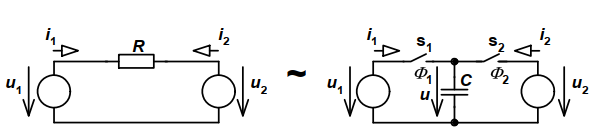
\includegraphics[scale=0.6]{images/SC.png}
   \end{center}
   \caption{Princip SC}
  \end{figure}
  
\begin{equation}
i=\frac{u}{R} \approx i_{ekv}=\frac{q}{T}=\frac{C*u}{T}=\frac{u}{R_{ekv}} => R_{ekv}=\frac{T}{C}
\label{eqn:i}
\end{equation}  

kde R je odpor, C je kapacita a T časová konstanta, q je náboj na kapacitoru, i\textsubscript{ekc} je celkový proud tekoucí
kapacitorem a u je celkové napětí na kapacitoru.

Rezistor, kterým protéká kontinuálně konstantní proud I lze nahradit spínačem s rezistorem. Z tohoto yplývá, že proud tekoucí kapacitorem má impulzní charakter (Obrázek \ref{fig:impulz}), tedy naprosto jiný, než je tomu u rezistoru. Pokud ale budeme uvažovat střední hodnotu těchto impulzů, která bude odpovídat rov. \ref{eqn:i}), je možné uvedené obvodové prvky nahradit.

   \begin{figure}[h]
   \begin{center}
     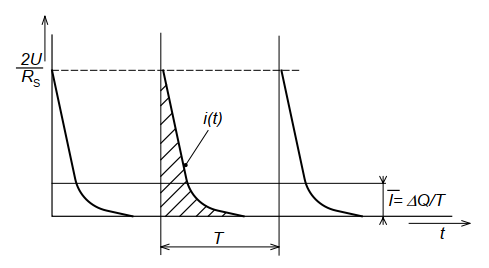
\includegraphics[scale=0.6]{images/Impulz.png}
   \end{center}
   \caption{Impulzní průběh SC}
   \label{fig:impulz}
  \end{figure}
  
  
\textbf{Z této náhrady vyplynulo několik výhod:} 
\begin{itemize}
\item na rozdíl od rezistoru, jehož výrobní chyba v IO je 5 až 20 \%, je přesnost
zpracování vstupního analogového signálu dána pouze přesností poměru kapacit,
která může být řádově až 0,01 \%,
\item  kapacitory je možné v technologii CMOS snadněji implementovat na čip,
\item  spínače CMOS mají v sepnutém stavu nízký odpor (řádu desítek ohmů),
\item  dobrá přesnost časových konstant,
\item  dobrá napěťová linearita
\item a dobré teplotní charakteristiky.
\end{itemize}

\textbf{Mezi nevýhody techniky SC patří} 
\begin{itemize}
\item pronikání řídicího hodinového signálu přes spínače do signálové cesty –
dochází ke znehodnocení zpracovávaného užitečného signálu,
\item injekce náboje ze spínače – dochází ke znehodnocení zpracovávaného
užitečného signálu,
\item  jednotlivé fáze řídicího hodinového signálu musí být realizovány jako
nepřekrývající se, což klade vysoké nároky na přesnost generovaného řídicího
hodinového signálu (viz. Obrázek \ref{fig:sig}),
\item chyby přizpůsobení použitých kapacitorů – negativně ovlivňují přesnost
převodu
\item a parazitní kapacity.
\end{itemize}
   \begin{figure}[h]
   \begin{center}
     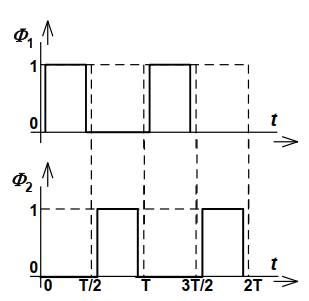
\includegraphics[scale=0.6]{images/SC_sig.png}
   \end{center}
   \caption{Řidicí a nepřekrývající se hodinové signály}
   \label{fig:sig}
  \end{figure}
\pagebreak
\subsubsection{Stejnosměrné přesné filtry}
Jsou vhodné jako antialiasingové filtry i jako filtry pro nepřímé převodníky. Kaskádní struktura filtru, však není pro realizaci příliš vhodná, protože se uplatňuje napěťová nesymetrie použitých OZ ve výstupním signálu. Jistým řešením je použití pasivních prvků, což způsobuje problémy při realizaci induktorů. Východiskem je tedy použití nekaskádní struktury aktivního filtru.

   \begin{figure}[h]
   \begin{center}
     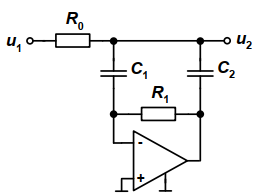
\includegraphics[scale=0.8]{images/Nekas.png}
   \end{center}
   \caption{Nekaskádní zapojení aktivního filtru 2. řádu}
   \label{fig:nekas}
  \end{figure}

\subsection{Důvody použití v převodnících}  
Plní hned několik funkcí, mezi které patří zejména potlačení aliasingu (záznějí), potlačení kvantovacího šumu na výstupu DAC a potlačení střídavých složek v nepřímých převodnících DA.
\subsection{Aproximační charakteristiky}

Filtry obecně nejsou specifikovány pouze mezními kmitočty, které definují propustné a zádržné oblasti. Důležitá je také zvolená aproximační metoda realizace filtru. V případě filtrů typu dolní propust existují čtyři základní aproximace, a to aproximace podle Butterwortha, Chebysheva (vč. inverzní verze) a Cauera (Darlingtona).

\textbf{Butterworthova aproximace} má maximálně plochou kmitočtovou charakteristiku kolem počátku a monotónně klesající průběh od mezního kmitočtu v nepropustném pásmu.

\textbf{Aproximace podle Chebysheva} je v propustném pásmu mírně zvlněná s monotónně klesající průběhem od mezního kmitočtu v nepropustném pásmu. 

\textbf{Inverzní Chebyshevova aproximace} má maximálně plochou kmitočtovou charakteristiku v propustném pásmu a pásmu potlačení je mírně zvlněná. 

\textbf{Aproximace Cauerova nebo také Darlingtonova} je mírně zvlněná v obou pásmech své kmitočtové charakteristiky. Proto se také pro ni ustálil výraz eleptický filtr.

   \begin{figure}[h]
   \begin{center}
     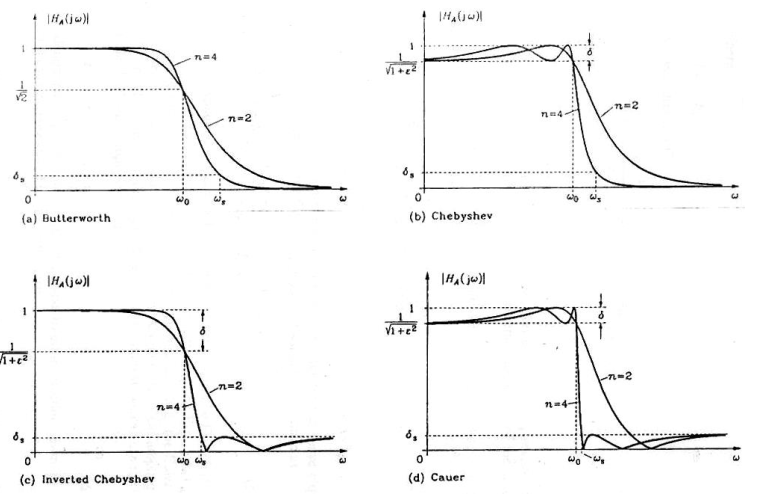
\includegraphics[scale=0.8]{images/Aprox.png}
   \end{center}
   \caption{Jednotlivé aproximace}
   \label{fig:sig}
  \end{figure}
\newpage 
\subsection{Přesné filtry}    
  Realizace filtru – ss přesné filtry
\begin{itemize}
\item výhodou těchto struktur je stejnosměrné oddělení všech
výstupů OZ pomocí kapacitorů od hlavní signálové cesty,
\item šum OZ se uplatňuje tím více, čím jsou blíže hlavní signálové
cesty => horní OZ nízkošumové,
\item filtr nesmí být zatěžován =>doplnit na výstupy vysoce kvalitní
oddělovací zesilovač.
\end{itemize}
Viz. Obrázek \ref{fig:nekas}.







\section{ZÁKLADY A TEORIE PŘESNÉHO NÁVRHU S OHLEDEM NA SOUBĚH PARAMETRŮ PRVKŮ INTEGROVANÉHO OBVODU}
Normální rozložení, Gaussova křivka, směrodatná odchylka, metoda Monte Carlo, princip superpozice (příklad součtu výstupních proudů z proudových zrcadel zatížených chybou souběhu)
\subsection{Normální rozložení}

\subsection{Gaussova křivka}
\begin{figure}[h]
   \begin{center}
     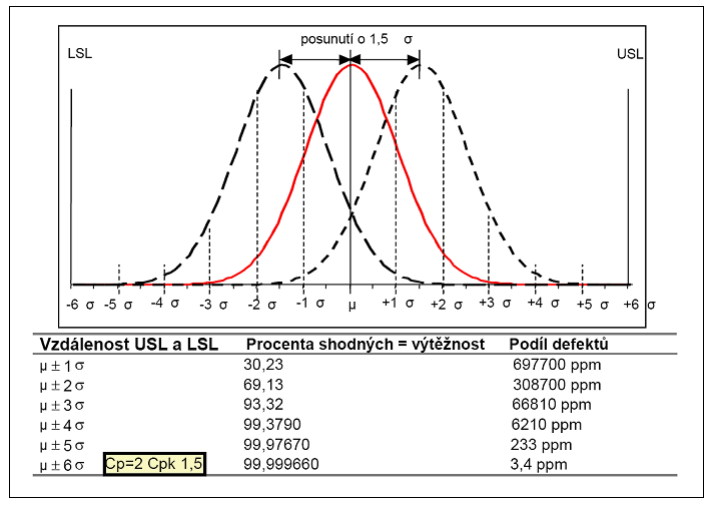
\includegraphics[scale=0.5]{images/Normal1.png}
   \end{center}
   \caption{Znázornění vlivu posunu procesu na ppm}
\end{figure}
\begin{figure}[h]
   \begin{center}
     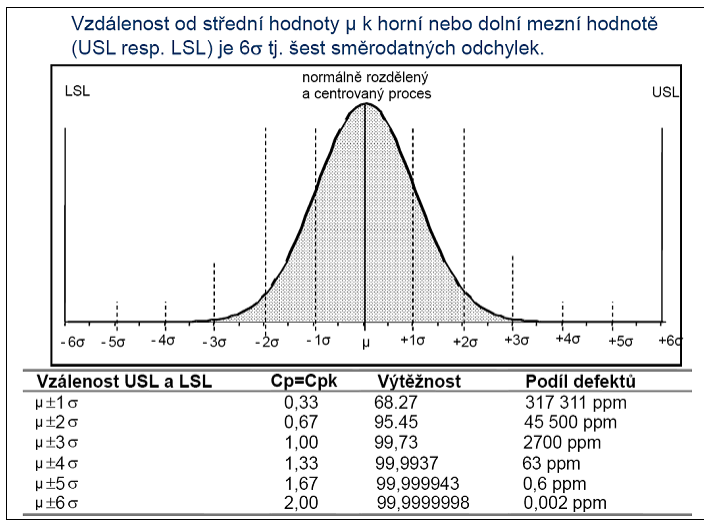
\includegraphics[scale=0.5]{images/Normal2.png}
   \end{center}
   \caption{Vycentrovaný proces a vliv na ppm}
\end{figure}
\subsection{Směrodatná odchylka}

\subsection{Metoda Monte Carlo}


\subsection{Princip superpozice}
Máme systém, který je charakterizován nějakou veličinou Q (např. offset, výstupní napětí,..). Chyba veličiny Q je dána několika dílčími nekorelovanými chybami uvnitř tohoto systému. Celková chyba veličiny Q se počítá tak, že se postupně vyjádří vliv každé dílčí chyby na veličinu Q, při tom se ostatní dílčí chyby zanedbají - položí rovno 0. NAkonec se vlivy všech dílcích chyb nekorelovaně sečtou a tím se získá celková chyba (rozptyl) veličiny Q.

\subsection{Příklad součtu výstupních proudů z proudových zrcadel}

\begin{figure}[h]
   \begin{center}
     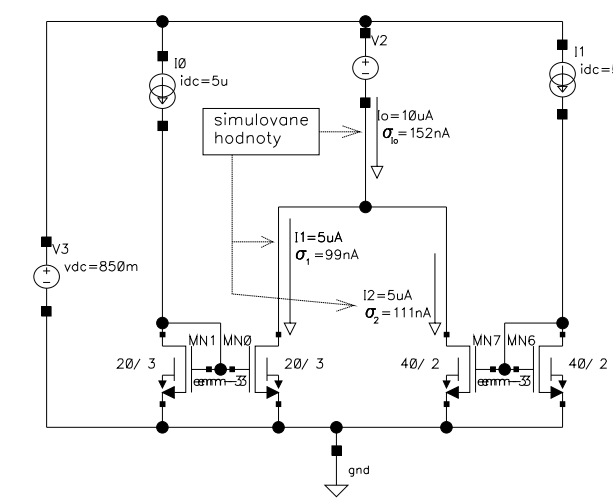
\includegraphics[scale=0.5]{images/Chyba_Souctu.png}
   \end{center}
   \caption{Chyba součtu dvou veličin}
\end{figure}

Mějme dvě veličiny I\textsubscript{1} a I\textsubscript{2}, které jsou vzájemně nekorelované (nijak na sobě nezávisí). Proud I\textsubscript{1} nikterak nezávisí na porudu I\textsubscript{2} a naopak. Velikost těchto proudů je zatížena chybou ($\sigma$\textsubscript{1} a $\sigma$\textsubscript{2}).

Chyba $\sigma$ součtu proudů se potom vypočítá jako:
\begin{equation}
\sigma = \sqrt{\sigma_{1}^{2}+\sigma_{2}^{2}}
\end{equation}

Při sčítání nekorelovaných veličin je jedna důležitá vlastnost. Pokud je jedna veličina menší než 1/2 největší veličiny, ve výsledku se téměř neprojeví (dá se zanedbat), protože zvýší výslednou hodnotu jen asi o desetinu.

Mějme: x\textsubscript{1}=1 a x\textsubscript{2} = 0,5. Potom:
\begin{equation}
\sigma = \sqrt{\sigma_{1}^{2}+\sigma_{2}^{2}}=\sqrt{1^{2}+0,5^{2}}=1,12\doteq 1
\end{equation}

\section{ZÁKLADNÍ VZTAHY PRO VÝPOČET CHYB V ANALOGOVÝCH OBVODECH }
Princip superpozice, celková chyba součtu a součinu dvou chybových veličin, přepočet chyb v obvodu diferenčního zapojení (výpočet vstupní napěťové nesymetrie komparátoru s BJT při známé chybě saturačního proudu vstupních tranzistorů)

\subsection{Princip superpozice}
Máme systém, který je charakterizován nějakou veličinou Q (např. offset, výstupní napětí,..). Chyba veličiny Q je dána několika dílčími nekorelovanými chybami uvnitř tohoto systému. Celková chyba veličiny Q se počítá tak, že se postupně vyjádří vliv každé dílčí chyby na veličinu Q, při tom se ostatní dílčí chyby zanedbají - položí rovno 0. NAkonec se vlivy všech dílcích chyb nekorelovaně sečtou a tím se získá celková chyba (rozptyl) veličiny Q.

\subsection{Příklad součtu výstupních proudů z proudových zrcadel}

\begin{figure}[h]
   \begin{center}
     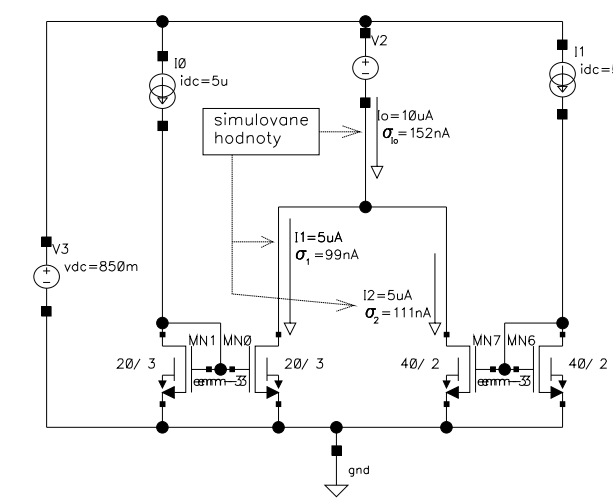
\includegraphics[scale=0.5]{images/Chyba_Souctu.png}
   \end{center}
   \caption{Chyba součtu dvou veličin}
\end{figure}

Mějme dvě veličiny I1 a I2, které jsou vzájemně nekorelované (nijak na sobě nezávisí). Proud I1 nikterak nezávisí na porudu I2 a naopak. Velikost těchto proudů je zatížena cyhbou ($\sigma$1 a $\sigma$2).

Chyba $\sigma$ součtu proudů se potom vypočítá jako:
\begin{equation}
\sigma = \sqrt{\sigma_{1}^{2}+\sigma_{2}^{2}}
\end{equation}

Při sčítání nekorelovaných veličin je jedna důležitá vlastnost. Pokud je jedna veličina menší než 1/2 největší veličiny, ve výsledku se téměř neprojeví (dá se zanedbat), protože zvýší výslednou hodnotu jen asi o deetinu.

Mějme: x1 = 1 a x2 = 0,5. Potom:
\begin{equation}
\sigma = \sqrt{\sigma_{1}^{2}+\sigma_{2}^{2}}=\sqrt{1^{2}+0,5^{2}}=1,12\doteq 1
\end{equation}

\subsection{Příklad součinu výstupních proudů z proudových zrcadel}

\begin{figure}[h]
   \begin{center}
     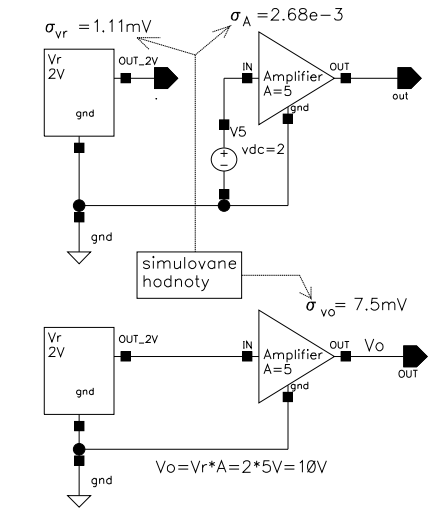
\includegraphics[scale=0.5]{images/Chyba_Soucinu.png}
   \end{center}
   \caption{Chyba součinu dvou veličin}
\end{figure}

Chyba $\sigma$vo výstupního napětí Vo se spočítá jako nekorelovaný součet vlivu těchto dvou dílčích chyb. Nejdříve předpokládejme, že chyba $\sigma$vr referenčního napětí je nulová, tedy že výsledná chyba je dána pouze chybou $\sigma$A zisku A. Výstupní napětí Vo1 a jeho chyba $\sigma$vo1 je potom:
\begin{equation}
V_{o1} = V_{r}*(A+\sigma_{A})=V_{r}*A+V_{r}*\sigma_{A}
\end{equation}

Výsledná chyba $\sigma$o výstupního napětí Vo je pak dána nekorelovaným součtem výše vypočítaných dílčích chyb:
\begin{equation}
\sigma_{o1} = \sqrt{\sigma_{vo1}^{2}+\sigma_{vo2}^{2}}=\sqrt{(V_{r}+\sigma_{A})^2+(A+\sigma_{vr})^2}
\end{equation}

Vztah pro $\sigma$vo lze zapsat i následovně:
\begin{equation}
\frac{\sigma_{vo}}{A*V_{r}}=\frac{\sigma_{vo}}{V_{o}}=\sqrt{(\frac{\sigma_{vr}}{V_{r}})^2+(\frac{\sigma_{vr}}{A})^2}
\end{equation}

Tedy, že relativní normovaná chyba součinu dvou veličin zatížených chybami je dána nekorelovaným součtem relativních chyb jednotlivých složek součinu.

\subsection{Přepočet chyb v obvodu diferenčního zapojení}

\begin{figure}[h]
   \begin{center}
     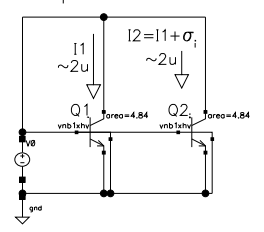
\includegraphics[scale=1]{images/Prepocet.png}
   \end{center}
   \caption{Chyba vstupního proudu}
\end{figure}

Měření probíhá na teoreticky identických tranzistorech Q1 a Q2. Měřením je zjištěn rozdíl proudů (odchylky), kdy z této ochylky můžeme spočítat chybu $\sigma$I1/I2 poměru proudů I1 a I2:
\begin{equation}
I_{2} = I_{1}+\sigma_{1} => \frac{I_{2}}{I_{1}} = \frac{I_{1}+\sigma_{i}}{I_{1}}=1+\frac{\sigma_{i}}{I_{1}} => \frac{\sigma_{i}}{I_{1}} = \sigma_{I1/I2}
\end{equation}

Z tohoto výpočtu potom můžeme na základě úvahy "o kolik musíme změnit Ube tranzistoru Q1, aby proud I1 byl stejný jako proud I2" určit nesouběh Ube dvou identických tranzistorů. Jinak řečeno, určíme rozdíl Ube těchto dvou tranzistorů pro případ, kdy hodnota proudu I2 je přesně rovna prudu I1:
\begin{equation}
\sigma_{dUbe} = U_{T}*ln(1+\sigma_{I1/I2})
\end{equation}

\begin{figure}[h]
   \begin{center}
     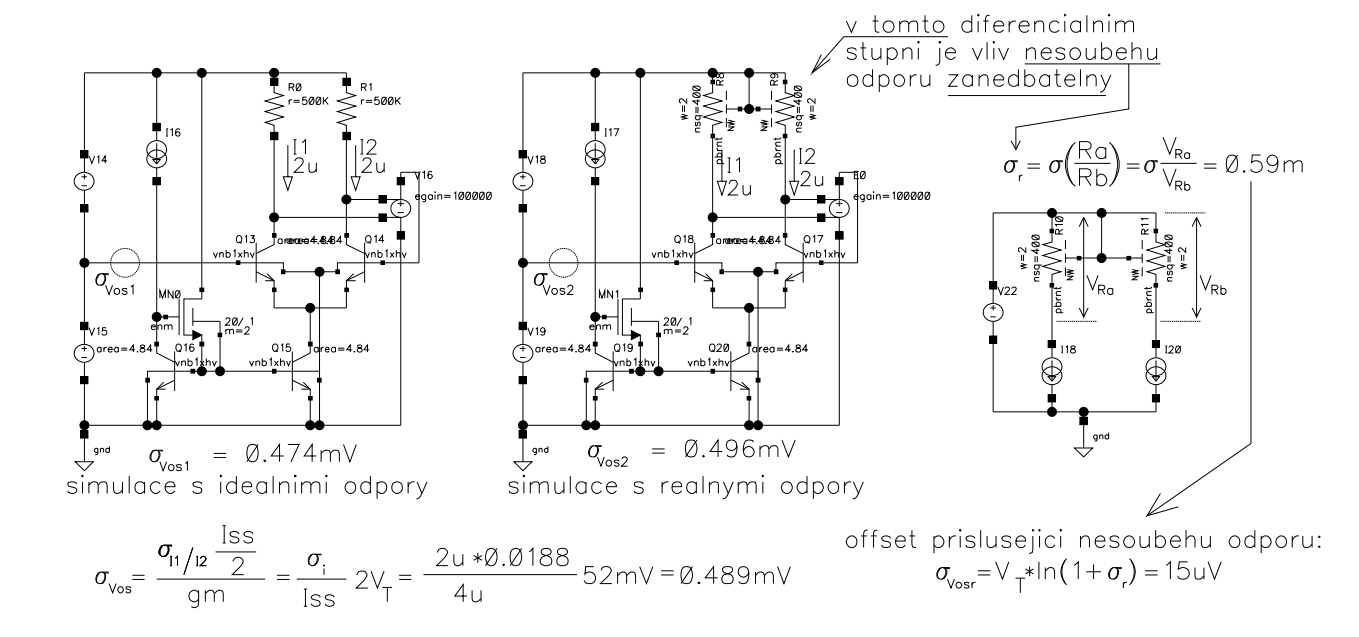
\includegraphics[scale=0.4]{images/Soubeh.png}
   \end{center}
   \caption{Reálná simulace nesymetrie}
\end{figure}


























\section{PŘESNÁ TRANZISTOROVÁ DVOJICE}
Souběh, proudové zrcadlo, diferenční stupeň, vliv rozměrů MOS tranzistorů na přesnost, Pelgromova rovnice

\subsection{Proudové zrcadlo}
\begin{figure}[h]
   \begin{center}
     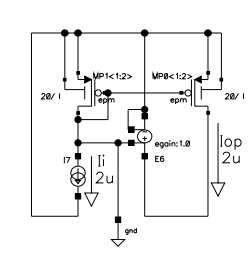
\includegraphics[scale=0.6]{images/MOS1.png}
   \end{center}
   \caption{Proudové zrcadlo}
\end{figure}

Proudové MOS zrcadlo (např. pro aktivní zátěž) navrhneme jako dvojici PMOS tranzistorů s danou šířkou kanálu W. Úkolem je poté najít takovou délku L, při níž chyba $\sigma$\textsubscript{Iop} této aktivní zátěže bude menší, než chyba vypočítaná pro diferenciální stupeň (např. 19 nA).

\begin{figure}[h]
   \begin{center}
     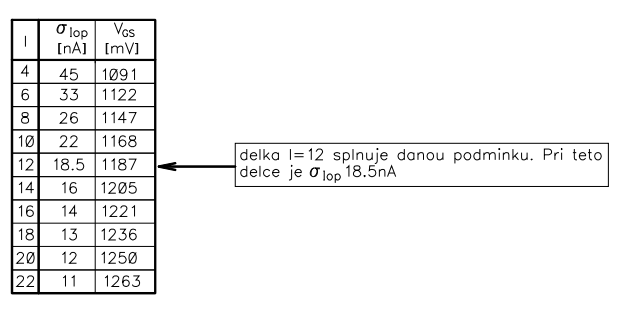
\includegraphics[scale=0.6]{images/Urceni.png}
   \end{center}
   \caption{Určení Ugs na základě chyby}
\end{figure}

\subsection{Diferenční stupeň}
\begin{figure}[h]
   \begin{center}
     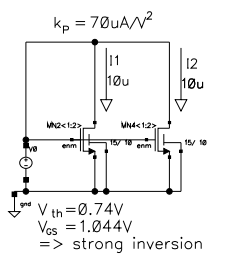
\includegraphics[scale=0.6]{images/MOS6.png}
   \end{center}
   \caption{Zapojení pro získání nesouběhu dif. stupně}
\end{figure}

Toto je základní zapojení pro měření nesouběhu dvou identických tranzistorů. Ze změřené hodnoty  chyby $\sigma$I\textsubscript{1}/I\textsubscript{2} proudu I\textsubscript{1} a I\textsubscript{2} je potom možné spočítat chybu$\sigma$\textsubscript{dVGS} souběhu V\textsubscript{GS} těchto dvou tranzistorů.
\begin{equation}
I_{2}/I_{1} = 1
\end{equation}
\begin{equation}
\sigma_{i}=\sigma_{I1/I2}*I1
\end{equation}
\begin{equation}
\sigma_{dVGS}=\frac{\sigma_{i}}{gm}
\end{equation}

Nesouběh $\sigma$\textsubscript{dVGS} dvou V\textsubscript{GS} napětí tranzistorové dvojice se projeví jako vstupní offset $\sigma$\textsubscript{VGS} elementárního operačního zesilovače.
\newpage
\subsection{Vliv rozměrů MOS tranzistorů na přesnost}
\begin{figure}[h]
   \begin{center}
     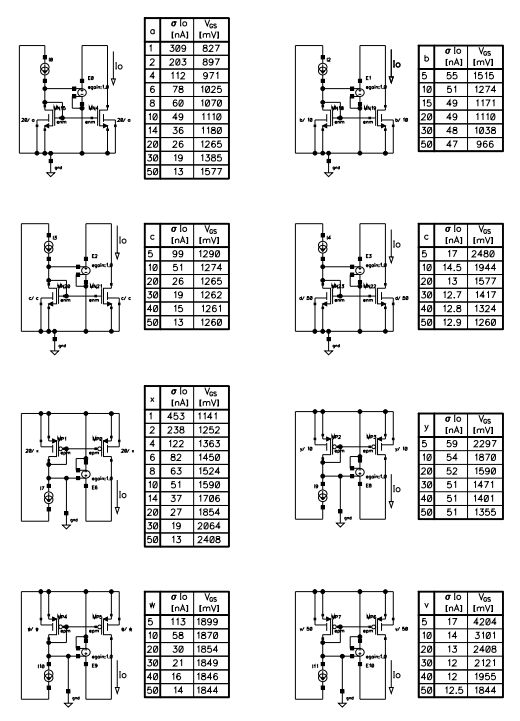
\includegraphics[scale=0.8]{images/Presnost.png}
   \end{center}
   \caption{Určení chyby na základě určení rozměrů MOS tranzistorů}
\end{figure}

\subsection{Pelgromova rovnice}
\begin{equation}
\sigma_{\Delta Id/Id}^2=\sigma_{UT0}^2*\frac{4}{(U_{GS}-U_{T0})^2}+\sigma_{\Delta \beta / \beta}^2
\end{equation}

kde chyba v U\textsubscript{T0}:
\begin{equation}
\sigma_{UT0}^2*\frac{4}{(U_{GS}-U_{T0})^2}
\end{equation}
a chyba v matchingu $\beta$:
\begin{equation}
\sigma_{\Delta \beta / \beta}^2
\end{equation}

Pro dobrý matching (malý proudový rozdíl) je dobré volit velké MOS (velké WL) a větší (U\textsubscript{GS} - U\textsubscript{T0})

\begin{figure}[h]
   \begin{center}
     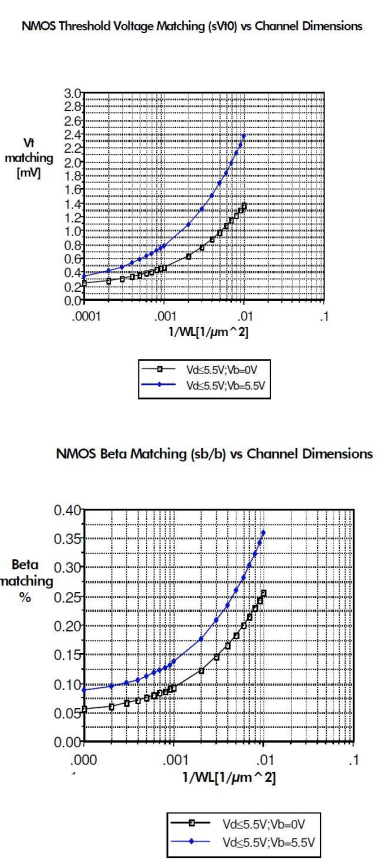
\includegraphics[scale=0.8]{images/grafy.png}
   \end{center}
   \caption{Threshold a Beta matching v závislosti na rozměrech kanálu}
\end{figure}


















\section{Sériové převodníky DA}
- základní zapojení a funkce, využití kapacitorů v síti, příklady využití

\subsection{Základní zapojení a funkce}
Sériové převodníky DA zaujímají zvláštní pozici mezi převodníky, v integrované podobě se prakticky nevyrábějí. Ve srovnání s paralelním převodníkem obsahuje pouze tři přesné analogové obvody, analogovou sčítačku, analogovou děličku a analogovou paměť.
\begin{figure}[h]
   \begin{center}
     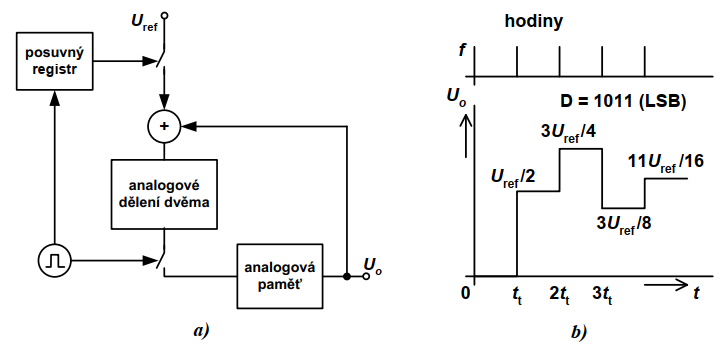
\includegraphics[scale=0.6]{images/DAser.png}
   \end{center}
   \caption{Zapojení sériového DAC}
\end{figure}

Pracují na principu postupného řízeného kvantování referenčního napětí číslicovým
signálem a sčítání váhových kvant jednotlivých bitů číslicového signálu. Sériový číslicový signál D\textsubscript{S} řídí horní spínač, který při D\textsubscript{S} = 1 připojuje kladné referenční napětí U\textsubscript{ref} do analogové sčítačky. Ve sčítačce se toto napětí sčítá s napětím u\textsubscript{k-1}, jež je udržováno na výstupu analogové paměti jako výsledek předchozího taktu převodu T\textsubscript{k-1}. Součet napětí se dělí dvěma a uloží opět do analogové paměti. Vstupní n-bitové číslo se tedy převede na analogový signál postupně, a to celkem v n taktech. Převod začíná od bitu s nejnižší vahou.

\subsection{Využití kapacitorů v síti, příklady využití}
\subsubsection{Sériový DAC s vybíjením kapacitoru}
Využívá exponenciální závislosti mezi impulzy v sériově vyjádřeném dvojkovém slově a exponenciálním tvarem vybíjecí křivky kapacitoru. Podle zjednodušeného schématu je kapacitor během první poloviny periody T/2 nabíjen ze zdroje konstantního proudu IC, pokud je však hodnota převáděného bitu rovna 1.

Protože kapacita C i proud IC jsou konstantní, bude také konstantní náboj dodaný do kapacitoru:
\begin{equation}
Q=I_{C}*\frac{T}{2}
\end{equation}
V průběhu doby T/2 napětí na kapacitoru lineárně narůstá a dosáhne hodnoty
\begin{equation}
U_{ref}=\frac{I_{C}}{C}*\frac{T}{2}
\end{equation}

\begin{figure}[h]
   \begin{center}
     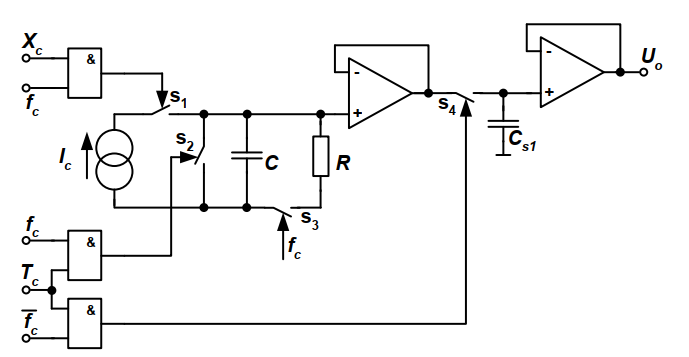
\includegraphics[scale=0.6]{images/DACC.png}
   \end{center}
   \caption{Sériový DAC s vybíjením kapacitoru}
\end{figure}

\begin{figure}[h]
   \begin{center}
     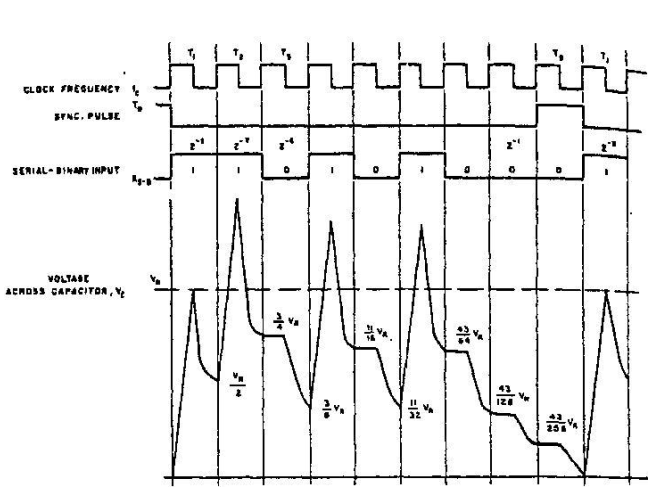
\includegraphics[scale=0.6]{images/DAgraf.png}
   \end{center}
   \caption{Příklad převodu dvojkového čísla 00101011}
\end{figure}
\newpage
\subsubsection{Sériový převodník s analogovými vzorkovači}
Sériový převodník s analogovými vzorkovači využívá rovněž metodu dělení napětí dvěma v jednotlivých taktech. 
\begin{figure}[h]
   \begin{center}
     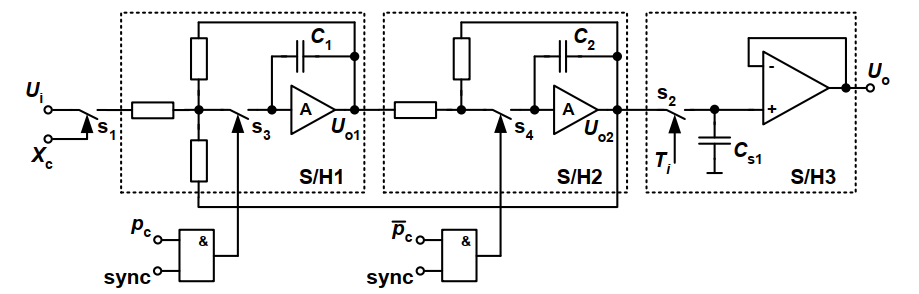
\includegraphics[scale=0.6]{images/DA2.png}
   \end{center}
   \caption{Sériový převodník s analogovými vzorkovači}
\end{figure}
Činnost každého vzorkovače může být rozčleněna do dvou fází – vzorkování a pamatování. Při sepnutých spínačích s\textsubscript{1} a s\textsubscript{3} bude vzorkovač S/H1 vzorkovat a jeho výstupní napětí se ustálí na hodnotě (je-li přenášený bit 1):
\begin{equation}
U_{o1}=-\frac{1}{2}*(U_{ref}+U_{o2})
\end{equation}
Toto vzorkování je podmíněno koincidencí hodinových impulzů a synchronizačního signálu p\textsubscript{c}. sync (tedy vždy první polovina periody Ti až do signálu sync = 1). Ve druhé polovině periody Ti se přepne S/H1 do režimu pamatování a naopak S/H2 se sepnutím s\textsubscript{4} převede do režimu vzorkování.

Vzorkovač S/H2 má v režimu vzorkování přenos -1 a uloží do své analogové paměti napětí –U\textsubscript{o1} právě ukončené předchozí poloviny periody. Cyklickým pochodem se tak v každé periodě dělí původní napětí na polovinu. Sériovým převodem se při každé 1 na pozici bitu přičítá celé U\textsubscript{ref}.
\begin{figure}[h]
   \begin{center}
     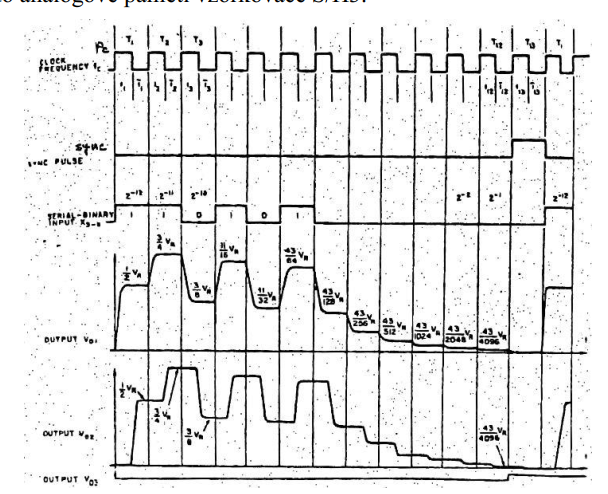
\includegraphics[scale=0.6]{images/DAgraf2.png}
   \end{center}
   \caption{Časové průběhy pro převod 12-bitového čísla na výstupní napětí}
\end{figure}

\pagebreak
\subsection{Sériový cyklický DAC s kapacitory}
Sériový cyklický DAC s kapacitory obsahuje jen dva přesné rezistory, tři paměťové kapacitory, dva OZ a napěťové spínače. Cyklický převodník je rychlejší než převodník se vzorkovači. Aktivace spínačů je symbolicky vyznačena přímou proměnnou pro aktivní 1 a invertovanou proměnnou pro aktivní 0.
\begin{figure}[h]
   \begin{center}
     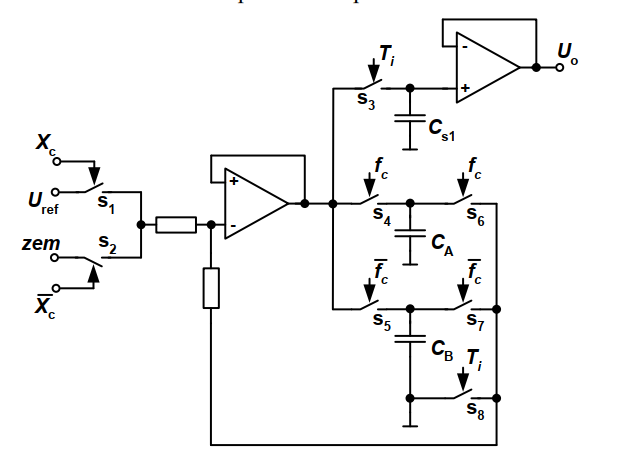
\includegraphics[scale=0.6]{images/DAser2.png}
   \end{center}
   \caption{Sériový cyklický DAC s kapacitory}
\end{figure}

Převáděné číslo je zpracováváno postupně od LSB, je-li bit = 1, spíná se s\textsubscript{1} a na vstup převodníku se přivede U\textsubscript{ref}. Pro bit s hodnotou 0 se sepnutím s2 připojí 0 V. Ostatní spínače jsou řízeny přímými nebo invertovanými signály f\textsubscript{c} (hodinové pravoúhlé impulzy), T\textsubscript{1} (identifikuje první takt) a T\textsubscript{12} (identifikuje konec převodu).

\subsection{Sériový DAC s vyrovnáním náboje}
Sériový DAC s vyrovnáním náboje využívá principu předávání (vyrovnání) náboje mezi nabitým a vybitým kapacitorem po jejich paralelním spojení. Napětí na obou spojených kapacitorech bude stejné a budou-li obě kapacity také stejné tj. C\textsubscript{1} a C\textsubscript{2}, budou stejné i oba náboje Q\textsubscript{1} = Q\textsubscript{2} a výsledné napětí bude přesně poloviční (Uref/2) proti napětí U\textsubscript{ref} původně plně nabitého kapacitoru. Vyrovnání náboje neproběhne ihned, ale s určitým zpožděním, které závisí na kapacitách C\textsubscript{1}, C\textsubscript{2} a na odporu R\textsubscript{s} sepnutého propojovacího spínače.
\begin{figure}[h]
   \begin{center}
     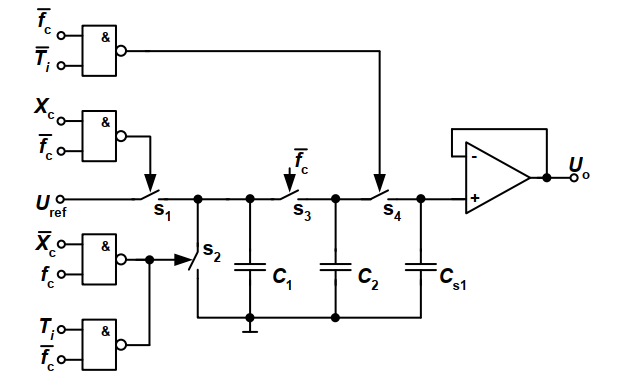
\includegraphics[scale=0.6]{images/DAvyrov.png}
   \end{center}
   \caption{Blokové zapojení sériového DAC s vyrovnáním náboje}
\end{figure}



\subsection{Nepřímé ADC}
Nepřímé převodníky DAC používají mezipřevod vstupní číslicové kombinace na jiný diskrétní signál, který je teprve převeden na výstupní analogový signál U(D). Tyto převodníky se klasifikují:
\begin{itemize}
\item vzorkováním periodických pilovitých kmitů (jedna z nejstarších metod),
\item podle druhu měronosné veličiny pomocného signálu se rozeznávají
\item nepřímé převodníky DA s mezipřevodem na poměr šířky a periody impulzů,
\item nepřímé převodníky DA s hustotou uniformních impulzů,
\item nepřímé převodníky DA s kmitočtem pravoúhlých kmitů.
\item s jiným typem mezipřevodu (magnetický modulátor, indukční dělič apod.).
\end{itemize}

V číslicově řízených kalibračních normálech napětí se užívají zejména DAC s mezi převodem na poměr šířky a periody impulzů (typicky 20-bitové převodníky). Na Obr. 96 je blokové schéma takového převodníku.
\begin{figure}[h]
   \begin{center}
     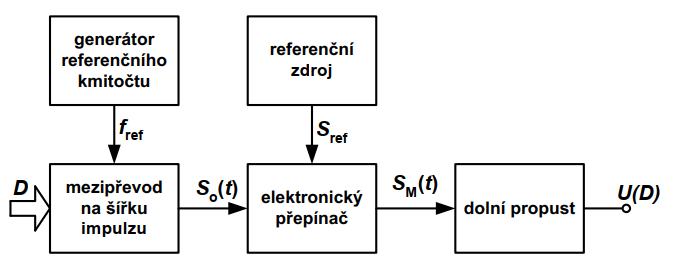
\includegraphics[scale=0.6]{images/DAneprimy.png}
   \end{center}
   \caption{Princip převodníku DAC s mezipřevodem na šířku impulzu}
\end{figure}







\section{Převodníky AD s vysokými vzorkovacími kmitočty}
- komparační, řetězové - základní zapojení a funkce, příklady využití.
\begin{figure}[h]
   \begin{center}
     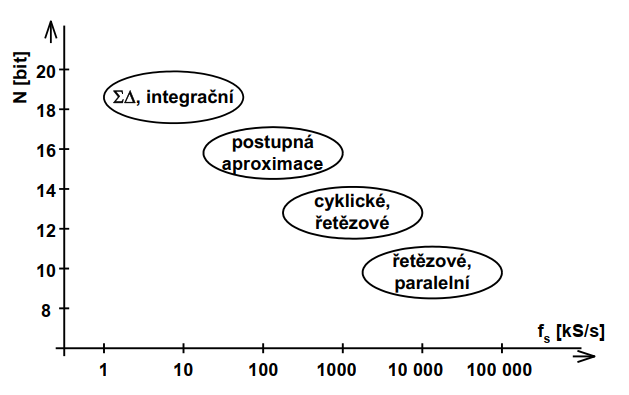
\includegraphics[scale=0.6]{images/ADroz.png}
   \end{center}
   \caption{Rozdělení ADC podle rozlišení v závislosti na četnosti převodu}
\end{figure}
\begin{figure}[h]
   \begin{center}
     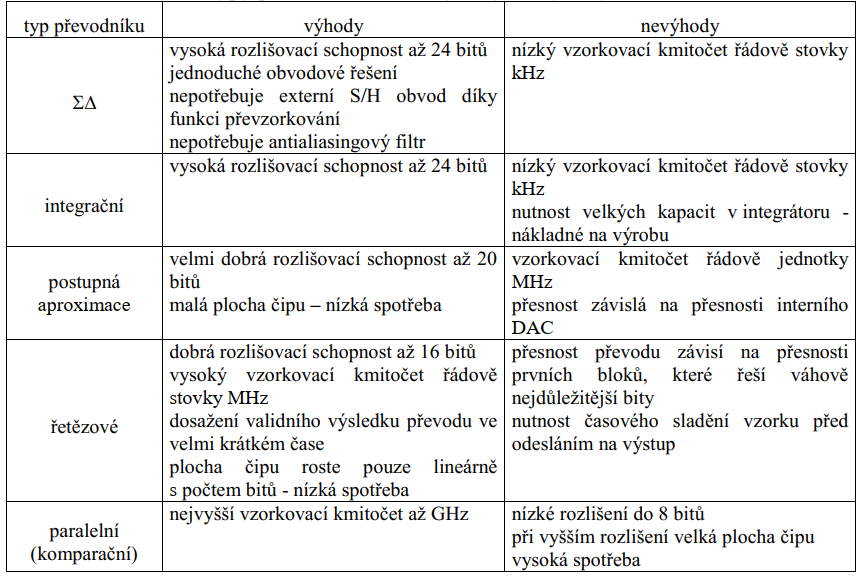
\includegraphics[scale=0.6]{images/ADroztab.png}
   \end{center}
   \caption{Základní typy převodníků AD – výhody, nevýhody}
\end{figure}
\subsection{Komparační}
Využívají přímou komparaci kvantovaného měřeného a referenčního napětí. Mohou dosáhnout extrémně krátké doby převodu. 

Nevýhodou je velký počet komparátorů a složitost dekodéru, uplatňující se u vícebitových převodníků. 

Kompenzační převodníky AD pracují na základě kompenzace měřeného napětí výstupním napětím řízeného převodníku DA. Z hlediska způsobu generace kompenzačního napětí lze rozlišovat ještě kompenzační převodníky s přírůstky kompenzačního napětí shodné a odstupňované velikosti. Integrační převodníky AD využívají řízené integrace měřeného a referenčního napětí, umožňují dosáhnout vysoké přesnosti převodu.

\textbf{Přímé převodníky AD} převádějí vstupní analogové napětí přímo na výstupní slovo. 

U \textbf{nepřímých převodníků AD} je vstupní analogové napětí převedeno nejprve na jinou analogovou veličinu (např. čas, kmitočet) a teprve potom je tato pomocná analogová veličina převedena do číslicového tvaru.
\begin{figure}[h]
   \begin{center}
     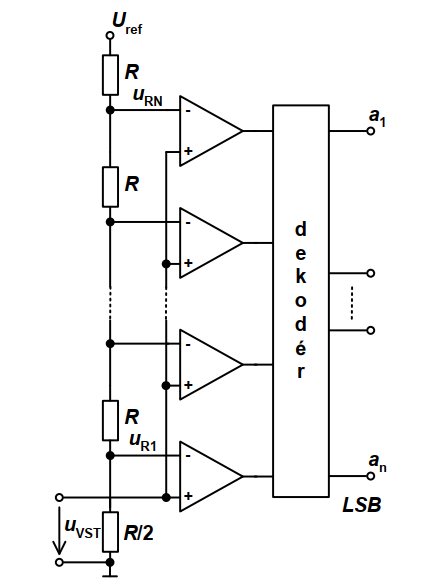
\includegraphics[scale=0.6]{images/ADkomp.png}
   \end{center}
   \caption{Zapojení paralelního komparačního převodníku AD}
\end{figure}

U paralelního typu je vstupní signál přiveden paralelně na řadu komparátorů. Na každý komparátor je rovněž připojena poměrná část referenčního napětí získaná na rezistorovém děliči zhotoveném z řady shodných rezistorů s odpory R. Pro každou možnou kvantovací hladinu existuje příslušná napěťová komparační úroveň. Komparační úrovně jsou v souladu s převodní charakteristikou  voleny do středu intervalů mezi jednotky vstupního napětí. Proto se například napětí u$\in$(2,5; 3,5 V) vyhodnotí aritmeticky správně, u = 3 V. Posun o polovinu kvantovacího bloku je docílen spodním rezistorem s odporem R/2 v rezistorové síti převodníku.

Přivede-li se libovolné dovolené vstupní napětí, všechny komparátory srovnávají jeho hodnotu s kvantovacími hladinami. Tyto komparátory, jejichž referenční úroveň je menší než vstupní napětí, nastaví na svém výstupu úroveň 1, u ostatních komparátorů bude na jejich výstupech logická nula. Výstupy všech komparátorů jsou vedeny na dekodér, kde se získá paralelní výstupní kód.

Tento ADC je
extrémně rychlý. Jeho rychlost je prakticky limitována jen rekreační dobou komparátorů
a dekódovací logiky. Jeho složitost však exponenciálně roste s počtem bitů.

\subsection{Řetězové}
V zájmu zmenšení počtu komparátorů a dodržení velké rychlosti převodu byly vyvinuty řetězové převodníky AD.

Typický řetězový ADC se skládá z několika stejných bloků (stupňů), které jsou kaskádně propojeny za sebou. Každý stupeň převodníku se skládá ze vstupního vzorkovacího obvodu, subADC a subDAC. Princip funkce je pro všechny stupně stejný. Vstupní signál je kvantován, pomocí subADC převeden do binární podoby a jako částečný výstup je poslán do bloku korekce. Mezitím je však opět pomocí subDAC převeden zpět do analogové podoby a odečten od původního vstupního signálu. Výsledné residuum u\textsubscript{res}, je pak ještě zesíleno a odesláno do dalšího stupně. První bloky tedy řeší nejvýznamnější bity (MSB) převodu, naopak nejméně významné bity řeší poslední blok, kterým je většinou jen několikabitový paralelní převodník.
\begin{figure}[h]
   \begin{center}
     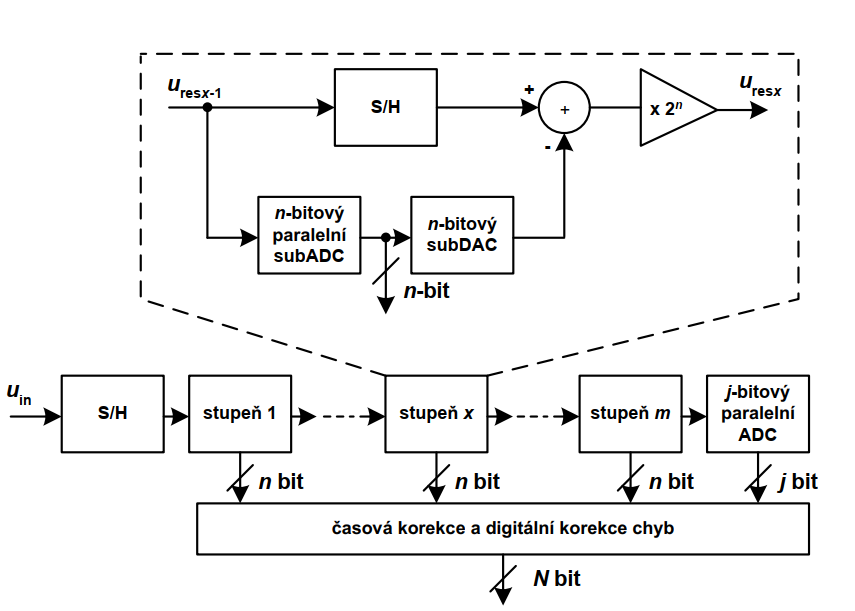
\includegraphics[scale=0.6]{images/ADret.png}
   \end{center}
   \caption{Princip řetězového ADC}
\end{figure}

\pagebreak
MDAC má rozlišení 1,5 bitu, což je nejčastěji používané rozlišení, a to
z několika důvodů. Při tomto rozlišení je dosaženo maximální šířky pásma a při zesílení 2
uzavřené smyčky je malá kapacitní zátěž a velký faktor zpětné vazby. Při tomto rozlišení
nedochází ani k degradaci celkové linearity převodu a SNR v důsledku nesymetrie
komparátoru. Navíc čím vyšší je rozlišení na stupeň, tím větší je i spotřeba obvodu.
\begin{figure}[h]
   \begin{center}
     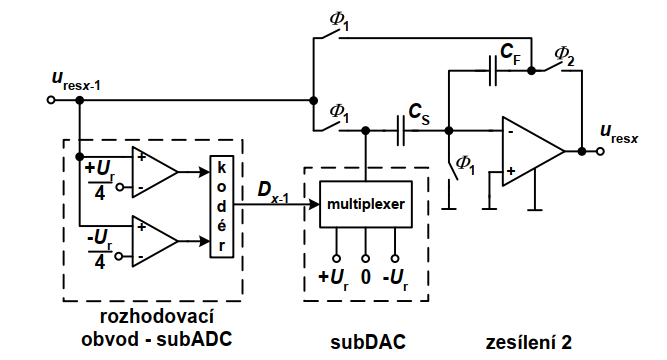
\includegraphics[scale=0.6]{images/MADC.png}
   \end{center}
   \caption{MDAC realizovaný technikou SC}
\end{figure}
\begin{figure}[h]
   \begin{center}
     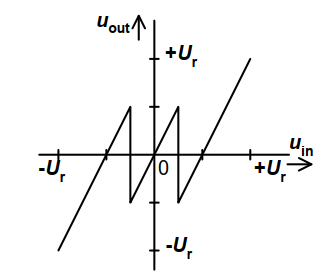
\includegraphics[scale=0.6]{images/MADCprev.png}
   \end{center}
   \caption{Převodní charakteristika 1,5-bitového MDAC}
\end{figure}

\pagebreak
\textbf{Použití:} v bateriově napájených zařízeních, dále v medicíně, komunikačních modulech apod.





\section{ŠUM}
Definice šumové hustoty a integrální hodnoty šumu a jejich vzájemný vztah, korelovaný a nekorelovaný příspěvek šumu, šumová charakteristika aktivních prvků (bílý a 1/f šum)
\section{Převodníky sigma-delta}
- základní zapojení a funkce, příklady využití.

Základní koncepce převodníků sigma-delta
\begin{itemize}
\item převzorkování měřeného signálu (oversampling) s převzorkovacím koeficientem OSR,
\item tvarování šumového signálu za účelem dalšího potlačení (noise-shaping) a zvýšení SNR a tím i zvýšení počtu bitů,
\item číslicová filtrace (digital filtering),
\item decimace.
\end{itemize}

Blok H(z) je integrátor, který se chová jako diskrétní filtr. Kvantovací obvod generuje digitální výstup y[k], který je tvořen součtem výstupu integrátoru y\textsubscript{h}[k] a kvantovací chyby e\textsubscript{q}[k]. Diskrétní filtr je obtížné analyzovat díky nelineárnímu chování kvantovacího obvodu. Jednou z metod, jak dosáhnout použitelných výsledků, je
nahrazení skutečného kvantovacího obvodu jeho lineárním modelem. Tato linearizace je použita k vysvětlení funkce modulátoru sigma-delta. 
\begin{figure}[h]
   \begin{center}
     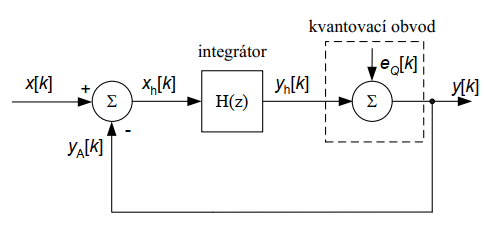
\includegraphics[scale=0.6]{images/sigma.png}
   \end{center}
   \caption{Blokové schéma lineárního modelu modulátoru sigma-delta}
\end{figure}

Signálová přenosová funkce (STF) a šumová přenosová funkce (NTF):
\begin{equation}
STF = \frac{H(z)}{1+H(z)}
\end{equation}

\begin{equation}
NTF = \frac{1}{1+H(z)}
\end{equation}

Jestliže je integrátor zvolen tak, že má mít vysoký zisk ve zpracovávaném pásmu f\textsubscript{B} a malý zisk mimo zpracovávané pásmo f\textsubscript{B}, pak se \textbf{STF} blíží 1 ve zpracovávaném pásmu. Mimo zpracovávané pásmo se STF blíží 0. 

Na druhou stranu, zisk \textbf{NTF} se blíží 0 ve zpracovávaném pásmu a 1 se blíží mimo zpracovávané pásmo. 

Diskrétní model integrátoru sigma-delta s jedním integrátorem je popisován jako modulátor sigma-delta prvního řádu. Zvyšováním řádu dochází k problému nestability modulátoru sigma-delta. Lineární model nemůže předpovídat, zda bude modulátor stabilní (nelze předpovídat, jestli póly reálného systému jsou uvnitř jednotkové kružnice = kritérium stability). V lineárním modelu je kvantovací obvod nahrazován jako konstantní zisk.
\begin{figure}[h]
   \begin{center}
     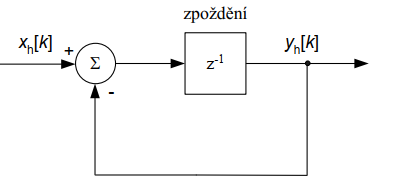
\includegraphics[scale=0.6]{images/sigma_dis.png}
   \end{center}
   \caption{Diskrétní model integrátoru}
\end{figure}

\pagebreak
U reálného kvantovacího obvodu je zisk proměnný. Přesnost
lineárního modelu se zvyšuje se zvyšujícím se rozlišení kvantovacího obvodu. Avšak jediná cesta jak dokázat, že je modulátor sigma-delta stabilní, je použití počítačové simulace.

Při návrhu modulátoru sigma-delta se volí optimální volbou mezi poměrem převzorkování (OSR), rozlišením kvantovacího obvodu N a řádem modulátoru sigma-delta k.

\subsection{Modulátory sigma-delta prvního řádu}
Na výstupu modulátoru sigma-delta je výstupní posloupnost bitů (bitstream). Bitstream je 1-bitový signál. Digitální 1 představuje nejvyšší možnou výstupní hodnotu a 0 představuje nejnižší možnou výstupní hodnotu. Kvantovací chyba v každém kroku je velká, protože je použit kvantovací obvod pouze se dvěma úrovněmi, průměruje kvantovaný signál, a proto se výstup modulátoru shoduje s analogovým vstupem. Tato střední hodnota je vypočítána decimačním filtrem, který následuje za modulátorem. Časová řada na výstupu integrátoru roste a klesá podle hodnoty zpětné vazby DAC. 1-bitový výstup z ADC je tvořen posloupností jedniček a nul, která modulováním šířky a periody impulzu reprezentuje vstupní analogovou hodnotu.
\begin{figure}[h]
   \begin{center}
     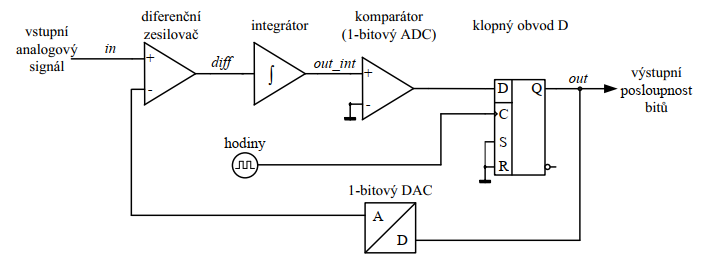
\includegraphics[scale=0.6]{images/sigmajedna.png}
   \end{center}
   \caption{Modulátor sigma-delta prvního řádu}
\end{figure}

Rozlišení modulátoru se zvyšuje s růstem počtu průměrovaných vzorků. To odpovídá růstu OSR. Na druhou stranu se snižuje šířka zpracovávaného pásma, a proto se musí volit kompromis mezi rozlišením a časem.

\subsection{Modulátory sigma-delta vyššího řádu}
Počet integrátorů v přímé větvi lze obecně libovolně zvyšovat, ale s tím narůstají problémy se stabilitou obvodu. Na případu jednoduché soustavy se zpětnou vazbou s více integrátory v přímé větvi si lze představit zdroj těchto problémů. Nestabilita modulátoru vyššího řádu nastane, pokud dojde k přetížení kvantovacího obvodu. Nestabilita nastává, když je vstup kvantovacího obvodu vybuzen vstupním signálem s vysokou amplitudou a nízkým kmitočtem.

Ve struktuře modulátoru sigma-delta jsou často používány integrátory se spínanými kapacitory a to ze dvou důvodů. Za prvé, přesnost koeficientů je určena poměrem kapacitorů, které je možné dosáhnout v technologii MOS s velkou přesností. Za druhé, hodnoty koeficientů nejsou závislé na vzorkovacím poměru, který je možné potom jednoduše změnit.
\begin{figure}[h]
   \begin{center}
     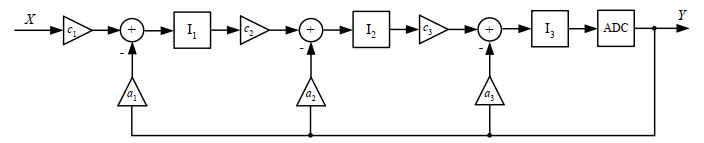
\includegraphics[scale=0.6]{images/sigmamulti.png}
   \end{center}
   \caption{Příklad modulátoru sigma-delta vyššího řádu}
\end{figure}

\subsection{Modulátory sigma-delta typu MASH}
U převodníků sigma-delta vyšších řádů byl velký problém se zajištěním stability celé soustavy. Řešením je paralelní zapojení jednoduchých modulátorů sigma-delta označováné jako převodník sigma-delta typu MASH (Multi Stage Noise Shaper).

\subsection{Sigma-delta převodník AD s filtrem typu pásmová propust}

Sigma-delta převodník AD s filtrem typu pásmová propust (bandpass filter) není tak známý jako jeho tradiční varianta, kdy je na výstupu připojen filtr typu dolní propust, nicméně jedná se o zapojení, které je poměrně často využíváno pro přímý převod komplexního analogového signálu na číslicový signál reprezentující amplitudu a fázi.

Tento typ převodníku je vhodný pro demodulaci kvadraturních, amplitudově modulovaných (QAM) signálů, tedy v GPS/GSM komunikačních systémů.

Bloková struktura modulátoru, která je tvořena bandpass filtrem, N-bitovým kvantovacím obvodem a číslicově-analogovým převodníkem zapojeným ve zpětné vazbě. Souvislost mezi kmitočtem vstupního signálu fin a hodinovým kmitočtem (f\textsubscript{s} = 4. fin) způsobuje, že je převodník fázově citlivý. Proto je nutné použít dva digitální filtry typu dolní propust Bandpass filtr lze syntetizovat pomocí kaskádního zapojení dvou nebo více bikvadraturních filtrů či rezonátorů, které musí mít ostrou převodní charakteristiku a jasně definovaný rezonanční kmitočet na kmitočtu f\textsubscript{n}. Tyto rezonátory lze implementovat jako diskrétní filtry využitím techniky spínaných kapacitorů nebo spínaných proudů.
\begin{figure}[h]
   \begin{center}
     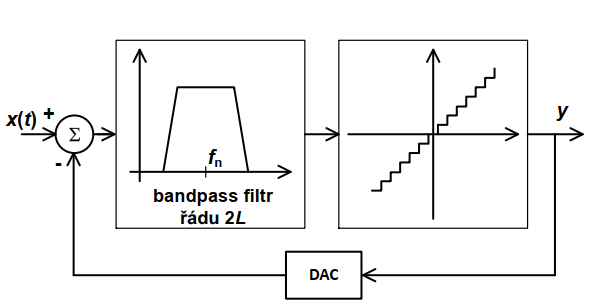
\includegraphics[scale=0.6]{images/sigmaBP.png}
   \end{center}
   \caption{Bloková struktura sigma-delta modulátoru s filtrem typu pásmová propust}
\end{figure}

\subsection{Převodníky DAC typu sigma-delta}
Tyto digitálně-analogové převodníky pracují na obdobném principu jako převodníky ADC typu $\Sigma$-$\Delta$. Blokové schéma obsahuje vstupní filtr, modulátor $\Sigma$-$\Delta$, jednobitový převodník DAC a výstupní antialiasingový analogový filtr. Ten vyhlazuje průběh výstupního signálu a odstraňuje nežádoucí vysokofrekvenční složky, které se do signálu dostaly vzorkováním a chybami digitálního řetězce.

\begin{figure}[h]
   \begin{center}
     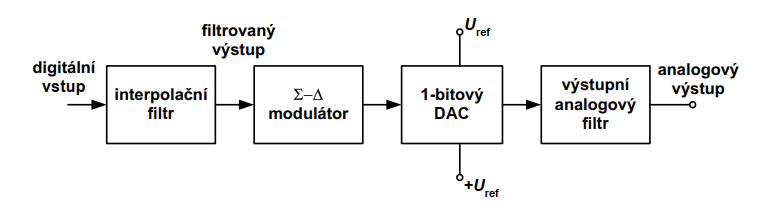
\includegraphics[scale=0.6]{images/sigmadac.png}
   \end{center}
   \caption{Příklad řešení převodníkem DAC typu $\Sigma$-$\Delta$}
\end{figure}

Rozdíl je však v implementaci. Vstupní filtr i modulátor $\Sigma$-$\Delta$ jsou digitální. Rozdíl
mezi hodnotami přicházejícího vzorku a číslicovou hodnotou reference (její polaritu řídí
vnitřní komparátor modulátoru) integrátor modulátoru integruje. Komparátor modulátoru
vyhodnocuje polaritu jeho výstupního signálu a podle ní ve vzorkovacích okamžicích připíná
na analogový výstup kladné nebo záporné analogové referenční napětí. Je-li vzorkování
dostatečně rychlé, odpovídá střední hodnota výstupního napětí digitální hodnotě vstupu. Zde
je nutné převzorkování. Čím přesnější má výstupní napětí být, tím je nutný delší interval pro
výpočet střední hodnoty, nebo tím vyšší musí být koeficient převzorkování.

Převzorkování společně s integrátorem modulátoru funguje jako antialiasingový filtr.
Ve výstupním řetězci je však signál číslicový a vstupní vzorky jsou k dispozici jen v určitých
okamžicích. Právě proto je tu vstupní digitální filtr výstupního řetězce (interpolační filtr).
Doplňuje ve vstupním proudu chybějící hodnoty, které jsou zapotřebí při převzokování.
Interpolační filtr dopočítává chybějící hodnoty pro převzorkování a odstraňuje tak ze
vstupního signálu všechny ty vysokofrekvenční složky, které se v digitální formě objevily digitalizací. Díky intermodulačnímu zkreslení a ještě dalším nelineárním zkreslením, se
mohou v použité části spektra objevit nepříjemné vedlejší efekty. Výstupní analogový filtr
vyhlazuje skokové změny analogového výstupu převodníku DAC. Bývá to analogový filtr
vyššího než druhého řádu.

\subsection{Decimační filtr}
V tradičních ADC pracující s Nyquistovým kmitočtem je kvantovací šum rozložen přes celé zpracovávané pásmo. Převodníky $\Sigma$-$\Delta$ pracují s pracovním kmitočtem několikanásobně vyšším než je Nyquistův kmitočet a kvantovací šum je rozložen do frekvenční oblasti přesahující rozsah zpracovávaného pásma
\begin{figure}[h]
   \begin{center}
     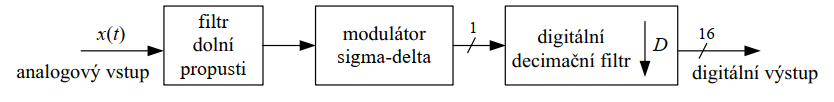
\includegraphics[scale=0.6]{images/sigmazak.png}
   \end{center}
   \caption{Základní systém převodníku sigma-delta}
\end{figure}

Díky filtraci výstupu modulátoru jsou tyto vysokofrekvenční složky odstraněny. Se vzrůstajícím řádem modulátoru dochází ke tvarování šumu, tak že kmitočtové spektrum je přesouváno do vyšších harmonických složek.

Funkcí decimačního filtru je odstranit šum z vyšších harmonických složek tak, aby nedošlo ke ztrátě signálu ve zpracovávaném pásmu. Další funkcí decimačního filtru je redukovat převzorkovaný výstupní signál modulátoru sigma-delta na signál s Nyquistovým kmitočtem. Návrh decimačního filtru závisí na digitálních koeficientech.
\newpage
\begin{figure}[h]
   \begin{center}
     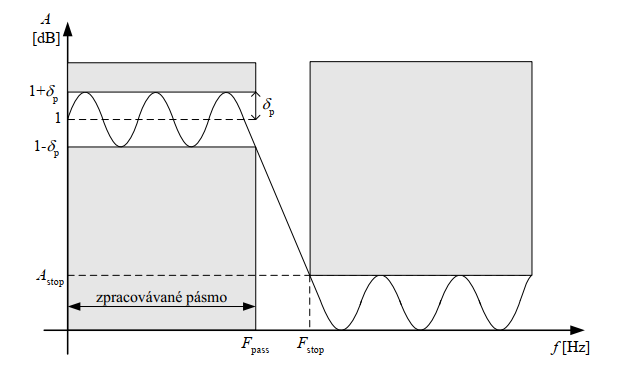
\includegraphics[scale=0.6]{images/decifiltr.png}
   \end{center}
   \caption{Kmitočtová charakteristika decimačního filtru}
\end{figure}

Kmitočet F\textsubscript{stop} je kmitočet, kdy dojde k zeslabení signálu na hodnotu A\textsubscript{stop}:
\begin{equation}
F_{stop}=\frac{F_{s}}{2*OSR}
\end{equation}























\section{OPERAČNÍ ZESILOVAČ}
- Buffer s jednotkovým zesílením\\
- Obecný koncový stupeň Rail-to-Rail\\
- Koncový stupeň Rail-to-Rail typu emitorový sledovač\\
- Operační zesilovač se stupněm typu složená kaskóda (folded cascode)\\

\end{document}
